% ------------------------------------------------------------------------
% bjourdoc.tex for birkjour.cls*******************************************
% ------------------------------------------------------------------------
%%%%%%%%%%%%%%%%%%%%%%%%%%%%%%%%%%%%%%%%%%%%%%%%%%%%%%%%%%%%%%%%%%%%%%%%%%

\documentclass{birkjour}
%
%
% THEOREM Environments (Examples)-----------------------------------------
%
 \newtheorem{thm}{Theorem}[section]
% \newtheorem{cor}[thm]{Corollary}
% \newtheorem{lem}[thm]{Lemma}
% \newtheorem{prop}[thm]{Proposition}
% \theoremstyle{definition}
 \newtheorem{defn}[thm]{Definition}
% \theoremstyle{remark}
% \newtheorem{rem}[thm]{Remark}
% \newtheorem*{ex}{Example}
 \numberwithin{equation}{section}

\usepackage[noadjust]{cite}
\usepackage{amsfonts}
\usepackage{listings}
\usepackage{algorithm}
\usepackage{algorithmic}

\begin{document}

%-------------------------------------------------------------------------
% editorial commands: to be inserted by the editorial office
%
%\firstpage{1} \volume{228} \Copyrightyear{2004} \DOI{003-0001}
%
%
%\seriesextra{Just an add-on}
%\seriesextraline{This is the Concrete Title of this Book\br H.E. R and S.T.C. W, Eds.}
%
% for journals:
%
%\firstpage{1}
%\issuenumber{1}
%\Volumeandyear{1 (2004)}
%\Copyrightyear{2004}
%\DOI{003-xxxx-y}
%\Signet
%\commby{inhouse}
%\submitted{March 14, 2003}
%\received{March 16, 2000}
%\revised{June 1, 2000}
%\accepted{July 22, 2000}
%
%
%
%---------------------------------------------------------------------------
%Insert here the title, affiliations and abstract:
%


\title[Rotation Estimation in Geometric Algebra]
 {Rotation Estimation in Geometric Algebra}

%----------Author 1
\author[Mauricio Cele Lopez Belon]{Mauricio Cele Lopez Belon}
\address{Buenos Aires, Argentina}
\email{mclopez@outlook.com}

%\thanks{This work was completed with the support of our \TeX-pert.}
%----------Author 2
%\author[Dietmar Hildenbrand]{Dietmar Hildenbrand}
%\address{Hochschule RheinMain, Ruesselsheim, Germany}
%\email{dietmar.hildenbrand@gmail.com}
%----------classification, keywords, date
\subjclass{Parallel algorithms 68W10; Clifford algebras, spinors 15A66}

\keywords{Geometric Algebra, Rotation Estimation, Wahba Problem}

\date{October 31, 2016}
%----------additions
%\dedicatory{To my wife}
%%% ----------------------------------------------------------------------

\begin{abstract}

We present a fast estimator of the rotation aligning two sets of corresponding vectors. Our method is faster than most conventional methods reported in literature, moreover it is robust to noise, accurate and simple to implement. It is based on minimizing a novel linear least squares error formulated in geometric algebra.

\end{abstract}

%%% ----------------------------------------------------------------------
\maketitle
%%% ----------------------------------------------------------------------
%\tableofcontents

The optimal rotation estimation from two sets of corresponding 3D vectors is a well known problem widely studied in linear algebra and quaternion algebra. On the other hand few work has been done on studying this problem using geometric algebra. Geometric algebra rotors are closely related to quaternions (quaternion algebra can be regarded as a geometric algebra defined on a set of imaginary basis vectors) we find geometric algebra to be a more natural choice for studying this problem since it is defined over a Euclidean vector space $\mathbb R^3$.

In this paper we introduce an efficient algorithm for estimating the best rotation aligning two sets of corresponding vectors. Our algorithm is faster than most conventional algorithms reported in literature. Our experiments demonstrate that it is robust to noise and accurate. Moreover, it is easy to implement. In fact, its implementation does not require access to any geometric algebra library, it can be implemented using any standard matrix and quaternion library. Our algorithm is based on minimizing a novel linear least squares error formulated in geometric algebra. Given the prevalence of quaternions in literature it is somewhat surprising to us that direct solution of the linear equations in quaternion form has never been exploited to derive algorithms such as the one presented, but that seems to be the case.

%In mathematics it is known as the Orthogonal Procrustes problem and is expressed in matrix algebra. In aeronautics it is known as Wahba's problem and it is solved mainly using quaternion algebra. In molecular chemistry it is known as Kabsch algorithm and is expressed in matrix algebra and in computer vision it is known as Absolute Orientation and solutions are expressed in matrix and quaternion algebra.

\section{Geometric Algebra $\mathbb{G}_3$}

A geometric algebra $\mathbb{G}_3$ is constructed over a real vector space $\mathbb R^3$, with basis vectors $\{e_1, e_2, e_3\}$. The associative geometric product is defined so that the square of any vector is a scalar $a a = a^2 \in \mathbb{R}$. From the vector space $\mathbb R^3$, the geometric product generates the geometric algebra $\mathbb{G}_3$ with elements $\{ X, R, A...\}$ called multivectors.

For a pair of vectors, a symmetric inner product $a \cdot b = b \cdot a$ and antisymmetric outer product $a \wedge b = -b \wedge a$ can be defined implicitly by the geometric product $a b = a \cdot b + a \wedge b$ and $b a = b \cdot a + b \wedge a$. It is easy to prove that $a \cdot b = \frac{1}{2}(a b + b a)$ is scalar, while the quantity $a \wedge b = \frac{1}{2}(a b - b a)$, called a bivector or $2$-vector, is a new algebraic entity that can be visualized as the two-dimensional analogue of a direction, that is, a planar direction. Similar to vectors, bivectors can be decomposed in a bivector basis $\{ e_{12}, e_{13}, e_{23} \}$ where $e_{ij} = e_i \wedge e_j$.

The outer product of three vectors $a \wedge b \wedge c$ generates a $3$-vector also known as the pseudoscalar, because the trivector basis consist of single element $e_{123} = e_1 \wedge e_2 \wedge e_3$. Similarly, the scalars are regarded as $0$-vectors whose basis is the number $1$. It follows that the outer product of $k$-vectors is the completely antisymmetric part of their geometric product: $a_1 \wedge a_2 \wedge ... \wedge a_k = \langle a_1 a_2 ... a_k \rangle_k$ where the angle bracket means $k$-vector part, and $k$ is its grade. The term grade is used to refer to the number of vectors in any exterior product. This product vanishes if and only if the vectors are linearly dependent. Consequently, the maximal grade for nonzero $k$-vectors is $3$. It follows that every multivector $X$ can be expanded into its $k$-vector parts and the entire algebra can be decomposed into $k$-vector subspaces:
\begin{equation*}
\mathbb G_3 = \sum_{k=0}^n{\mathbb{G}^k_3} = \{ X = \sum_{k=0}^n { \langle X \rangle_k } \}
\end{equation*}
This is called a \emph{grading} of the algebra. 

Reversing the order of multiplication is called reversion, as expressed by $(a_1 a_2 ... a_k)\tilde{} = a_k ... a_2 a_1$ and $(a_1 \wedge a_2 \wedge ... \wedge a_k)\tilde{} = a_k \wedge ... \wedge a_2 \wedge a_1$, and the reverse of an arbitrary multivector is defined by $\tilde{X} = \sum_{k=0}^n { \langle \tilde{X} \rangle_k }$.

Rotations are even grade multivectors known as rotors. We denote the subalgebra of rotors as $\mathbb{G}^{+}_3$. A rotor $R$ can be generated as the geometric product of an even number of vectors. A reflection of any $k$-vector $X$ in a plane with normal $n$ is expressed as the sandwitch product $(-1)^k n X n$. The most basic rotor $R$ is defined as the product of two unit vectors $a$ and $b$ with angle of $\frac{\theta}{2}$. The rotation plane is the bivector $B = \frac{a \wedge b}{\| a \wedge b \|}$.
\begin{equation*}
a b = a \cdot b + a \wedge b = \cos\left( \frac{\theta}{2} \right) + B \sin\left( \frac{\theta}{2} \right).
\end{equation*}
Rotors act on all $k$-vectors using the sandwitch product $X' = R X \tilde R$, where $\tilde R$ is the reverse of $R$ and can be obtained by reversing the order of all the products of vectors.

\section{Related Works}

\section{Geometric Algebra Rotor Estimation}

Given two sets of $n$ corresponding vectors $P = \{p_j\}_{j=1}^n$ and $Q = \{q_j\}_{j=1}^n$, we attempt to minimize the following error function:
\begin{eqnarray*}
E(R) = \min_{R \in \mathbb{G}^{+}_3 } \sum_j { c_{j} \|q_j - R p_i \tilde R\|^2 }\\
s.t. \ R \tilde R = 1
\end{eqnarray*}
where $\{c_{j}\}_{j=1}^n$ are scalar weights such that $\sum_j^n{c_j} = 1$. In that form, the minimization is a nonlinear least squares problem in $R$. Following Perwass, we can make it a linear least squares problem by multiplying by $R$ on the right and using the fact that $R \tilde R = 1$.
\begin{eqnarray*}
q_j - R p_j \tilde R = 0\\
q_j R - R p_j \tilde R R = 0\\
q_j R - R p_j = 0
\end{eqnarray*}
with the normalization constraint $R \tilde R = 1$ now implicit in the energy $E(R)$. Although the normalization is implicit, it is not enforced, so we will need to project $R$ back to the rotor manifold through normalization. So the equivalent linear least squares problem is:
\begin{eqnarray*}
E(R) = \min_{R \in \mathbb{G}^{+}_3 } \sum_j { c_{j} \|R p_j - q_j R\|^2 }\\
\end{eqnarray*}
Let $\Psi^j : \mathbb{G}^{+}_3 \mapsto \mathbb{G}^{-}_3$ be a function that maps even grade multivectors to odd grade multivectors. 
\begin{eqnarray*}
\Psi^j(R) = \sqrt{c_{j}} (R p_j - q_j R)
\end{eqnarray*}
And let $F^j : \mathbb{G}^{-}_3 \mapsto \mathbb{R}^4$ be a function that projects an odd grade multiverctor to a $4\times1$ column matrix.
\begin{eqnarray*}
F^j(X) = \left[\begin{array}{c} \langle X \rangle_1 \cdot e_1 \\ \langle X \rangle_1 \cdot e_2 \\ \langle X \rangle_1 \cdot e_3 \\ \langle X \rangle_3 \cdot \tilde I \end{array}\right]
\end{eqnarray*}
For the sake of simplicity we will refer to the composed function $F^j \circ \Psi^j:\mathbb{G}^{+}_3 \mapsto \mathbb{R}^4$ as simply $F^j$ with an abuse of notation.
Let $F$ be a column vector of $n$ functions $F^j$
\begin{eqnarray*}
F = \left[\begin{array}{c}F^1 \\ \vdots \\ F^n\end{array}\right]
\end{eqnarray*}
 such that the energy $E(R)$ can be expressed as matrix product
\begin{eqnarray*}
E(R) = F^T F =
\left[\begin{array}{ccc}F^{1T} & \cdots & F^{nT}\end{array}\right]
\left[\begin{array}{c}F^1 \\ \vdots \\ F^n\end{array}\right]
\end{eqnarray*}

The critical points of the energy $E(R)$ where it is minimized can be found solving $\nabla E(R) = 0$. Where the gradient has the following form:
\begin{eqnarray*}
g = \nabla E(R)\\
g = \nabla (F^T F)\\
g = 2 J^T F
\end{eqnarray*}
where $J$ is the Jacobian matrix of $F$. Since the energy $E(R)$ is purely quadratic in $R$, the solution for $\nabla E(R) = 0$ can be found by solving a linear system of equations. An optimal rotor is in the null space of a particular matrix derived from $J^T F = 0$. An easy way to obtain a solution in the null-space is using one iteration of Newton's method. Due to linearity of the equation $J^T F = 0$ w.r.t. $R$ one iteration suffice for obtaining a solution. The optimal increment for $E(R)$ is given by the Newton formula $\Delta R = H^{-1} \nabla E$, provided that the inverse of Hessian matrix $H^{-1}$ exists. Noting that $J$ does not depend on $R$, i.e. is constant, the Hessian matrix $H$ takes the simple form:
\begin{eqnarray*}
H = \frac{\partial(2 J^T F)}{\partial R} \\
H = 2 J^T \frac{\partial F}{\partial R}\\
H = 2 J^T J
\end{eqnarray*}
Where $H$ is independent of $R$. An optimal solution can then be found by solving a linear system.
\begin{eqnarray*}
R^* = R_0 - H^{-1} g(R_0)
\end{eqnarray*}
Where $R_0$ is an initial rotor and $g(R_0)$ is the gradient of $E$ evaluated at $R_0$. Of course, the choice of initial rotor $R_0$ has a particular effect on finding a local minimum. The energy $E(R)$ is non-convex, its shape is similar to a sinusoidal wave with infinitely many points at minimum energy value, each one at rotor $R_i = e^{-(\theta + i \pi) B}$ for $i \in \mathbb N$, being $B$ the optimal unique attitude bivector and $\theta $ an optimal angle with minimal absolute value. The choice of $R_0$ lead us to find a local solution close to it, the choice $R_0 = [1 \ 0 \ 0 \ 0]^T$ is optimal from the computational point of view and is also desirable because lead us to find solutions close to the \emph{identity} rotor. 

Since there are infinite solutions, $H$ is a singular matrix and consequently the problem is ill-posed. One simple solution is to use the Tikhonov regularization on $H$ to find an inverse $(H + \epsilon I)^{-1}$ that approaches the Moore-Penrose pseudo-inverse as $\epsilon$ approaches to zero. An optimal solution can then be found by solving a series of linear systems.
\begin{eqnarray*}
R_{i+1} = R_i - (H + \epsilon I)^{-1} g(R_i)
\end{eqnarray*}
until convergence is reached in the sense that $|R_i - R_{i+1}| < \xi$ for a small $\xi$. Where we use $R_0 = [1 \ 0 \ 0 \ 0]^T$. This algorithm has a number of advantages. Since Hessian $(H + \epsilon I)^{-1}$ is constant, it can be precomputed. Also the Jacobian matrix $J^T$ is constant, so it can be precomputed as well. But the computation of the gradient $g(R_i) = J^T F(R_i)$ is still required at each step. Although the computation of $g(R_i)$ is relatively cheap and this approach is fast we can do better by making the gradient constant as well.

\section{Fast Geometric Algebra Rotor Estimation}

From now on we will consider the gradient to be constant $g = g(R_0)$. Where $R_0 = [1 \ 0 \ 0 \ 0]^T$ is the identity rotor. However, we will add a very small regularization term to $E(R)$ to allow optimization. Our strategy is to introduce a new fixed rotor $R_i$ within a new function $\Phi(R, R_i) = \sqrt(\epsilon) (R - R_i)$. Let us define a function $D : \mathbb{G}^{+}_3 \mapsto \mathbb{R}^4$ that projects a multivector of even grade to a $4\times1$ column matrix.
\begin{eqnarray*}
D(X) = 
\left[\begin{array}{c} \langle X \rangle_0 \\ X \cdot e_{12} \\ X \cdot e_{13} \\ X \cdot e_{23}\end{array}\right]
\end{eqnarray*}
For the sake of simplicity we will refer to the composed function $D \circ \Phi:\mathbb{G}^{+}_3 \times \mathbb{G}^{+}_3 \mapsto \mathbb{R}^4$ as simply $D$ with an abuse of notation. The new term can be expressed as matrix product:
\begin{eqnarray*}
D^T D = \epsilon \|R - R_i\|^2
\end{eqnarray*}
with Jacobian 
\begin{eqnarray*}
J_D = \frac{\partial D}{\partial R} = \sqrt{\epsilon} I
\end{eqnarray*}
where $I$ is the $4\times4$ identity matrix. The energy now looks like this:
\begin{eqnarray*}
E_2(R, R_i) = F^T F + D^T D\\
E_2(R, R_i) = \sum_j { c_{j} \|R p_j - q_j R\|^2 } + \epsilon \|R - R_i\|^2
\end{eqnarray*}
Where $0 < \epsilon < 1$ is constant but small (we use $\epsilon = 10^{-6}$). The regularization term $D^T D = \epsilon \|R - R_i\|^2$ helps on finding a solution \emph{shifted} by a small amount towards the direction $\delta D = \epsilon (R - R_i)$, so one can interpret the rotor $R_i$ as a target of displacement. The regularization is perturbing the gradient and Hessian in the following way:
\begin{eqnarray*}
g_2 = \nabla(F^T F + D^T D)\\
g_2 = \frac{\partial (F^T F)}{\partial R} + \frac{\partial (D^T D)}{\partial R}\\
g_2 = 2 (J^T F + J_D^T D)\\
g_2 = 2 (J^T F + \sqrt{\epsilon} D)
\end{eqnarray*}
\begin{eqnarray*}
H_2 = 2 \frac{\partial(J^T F + \sqrt{\epsilon} D)}{\partial R} \\
H_2 = 2 J^T \frac{\partial(F)}{\partial R} + 2 \sqrt{\epsilon} \frac{\partial(D)}{\partial R}\\
H_2 = 2 (J^T J + \epsilon I)
\end{eqnarray*}
It is useful to express $g_2$ also as $g_2 = g(R) + \sqrt{\epsilon} D(R,R_i)$ and $H_2$ as $H_2 = H + \epsilon I$.  
An optimal solution can then be found by solving a series of linear systems:
\begin{eqnarray*}
R_{i+1} = R_0 - (H + \epsilon I)^{-1} (g(R_0) + \sqrt{\epsilon} D(R_0,R_i))
\end{eqnarray*}
This perturbation on the Hessian resembles now the Tikhonov regularization, and inverse $H_2^{-1}$ approaches the Moore-Penrose pseudo-inverse.
The perturbation on the gradient $g(R_0)$ affects its direction, forcing $R_{i+1}$ to move a little bit towards $R_i$.

Notice that if we take $R_i$ as being equal to $R_0$ then the gradient is not perturbed by any displacement. This is ok for finding an initial approximation $R_{i+1}$, moreover when the optimal rotor $R^*$ is close to $R_0$ the feedback is not necessary. However, if the optimal rotor is at $\pm \pi$ from $R_0$, that choice might cause the optimization get stuck. For example, given two sets of corresponding vectors $P = \{p_1=e1, p_2=e2\}$ and $Q = \{q_1=-e1, q_2=-e2\}$ which are rotated by $\pi$ radians to each other, the Hessian is diagonal, and its pseudo-inverse $H_2^{-1}$ is simply the reciprocal values of its diagonal, assuming $R_i = R_0$, the gradient $g(R_0)$ coincide with the first column of $H$, and so the product $H_2^{-1} g(R_0) = [1 \ 0 \ 0 \ 0]^T$ so the resulting rotor $R_{i+1} = R_0 - H_2^{-1} g(R_0) = [0 \ 0 \ 0 \ 0]^T$. In practice, we have never experienced this problem, even with synthetic data, since a tiny perturbation on the floating point precision is sufficient to get a non-zero $R_{i+1}$ which, after normalization, is useful as a feedback direction.

Given an estimated rotor $R_{i+1}$ a necessary condition for it to the optimal is that the recurrence $R_{i+1} = R_0 - H_2^{-1} g_2(R_0,R_i)$ converge to a rotor $R^*$ in the sense that $|R_i - R_{i+1}| < \xi$ for a small $\xi$. That is true because if $R_{i+1}$ is already optimal, the small displacement induced by the regularization term $\sqrt{\epsilon} D(R_0,R_i)$ should increase the least squares error $E_2$ and the linear system should compute the last $R_{i+1} = R^*$ as it has less error. So regularization term can be seen as a feedback for reaching a stable $R^*$. Since the regularization term is only affecting the gradient, the computation is very cheap. The gradient $g(R_0)$ can be precomputed as well as the matrix $H_2^{-1}$, and the iteration is reduced to compute a matrix vector multiplication.

%Given an estimated rotor $R_{i+1}$ we can check that $R_{i+1}$ is the optimal $R^*$ if we take $R_i$ as being equal to $R_{i+1}$ and solving again for $R_{i+1}$ gives us the same rotor, i.e., $R^*$. That is true because if $R^*$ is already optimal, the small displacement induced by the regularization term should increase the error $E(R^*)$ and the next value given by Newton formula should be $E(R^*)$ again. In the cases where the optimal rotor is far from $R_0$, the given rotor $R_{i+1}$ is probably not optimal, but repeating the Newton iteration a few times using $R_i = R_{i+1}$ (often one to three times) will eventually give an stable $R^*$. So regularization term can be seen as a feedback for reaching a stable minimal $R^*$. Since the regularization term is only affecting the gradient, the Newton iteration is very cheap. The reason is that the linear system need to be solved just once (i.e., we are inverting $H$ once) and the iteration is reduced to compute a matrix vector multiplication.

\section{Optimal Computation of Jacobians}

% Lets recall that each term of the sum $\sum_j { c_{j} \|R p_j - q_j R\|^2 }$ can be expressed in matrix form as function $F^{jT} F^j$ where:
% \begin{eqnarray*}
% F^j(R) = \sqrt{c_{j}} (R p_j - q_j R)
% \end{eqnarray*}
% $F^j$ is producing a multivector with the basis $\{ e_1, e_2, e_3, e_{123}\}$.
% Jacobian of $F^j$ is $\frac{\partial F^j}{\partial R}$:
% \begin{eqnarray*}
% J^j = \left[\begin{array}{cccc}\frac{\partial F^j}{\partial w} & \frac{\partial F^j}{\partial e_{12}} & \frac{\partial F^j}{\partial e_{13}} & \frac{\partial F^j}{\partial e_{23}}\end{array}\right]
% \end{eqnarray*}

% Solution to $H \Delta R = g(R_0)$ looks like this:
% \begin{eqnarray*}
% \left[\begin{array}{ccc}J^{1T} & \cdots & J^{nT}\end{array}\right]
% \left[\begin{array}{c}J^1 \\ \vdots \\ J_1^n\end{array}\right]
% \Delta R = 
% \left[\begin{array}{ccc}J^{1T} & \cdots & J^{nT}\end{array}\right]
% \left[\begin{array}{c}-F^1 \\ \vdots \\ -F^n \end{array}\right]
% \end{eqnarray*}

% \begin{eqnarray*}
% \left( \sum_j{J^{jT} J^j} \right) \Delta R = -\sum_j{J^{jT} F^j} 
% \end{eqnarray*}
% \begin{eqnarray*}
% R^* = R_0 + \Delta R
% \end{eqnarray*}
% where we should normalize the rotor $R^*$ for sending it back to the manifold.

% \subsubsection{Form of the Jacobians}

The differential of $F^j$ defined as $J^j = \frac{\partial F^j}{\partial R}$ is a $4\times4$ matrix which four columns are the directional derivatives of $F^j = \sqrt{c_j} (R p_j - q_j R)$ w.r.t rotor components on the basis $\mathbb{G}^{+}_3$:
\begin{eqnarray*}
J^j = \left[\begin{array}{cccc}\frac{\partial F^j}{\partial w} & \frac{\partial F^j}{\partial e_{12}} & \frac{\partial F^j}{\partial e_{13}} & \frac{\partial F^j}{\partial e_{23}}\end{array}\right]
\end{eqnarray*}
\begin{eqnarray*}
\frac{\partial F^j}{\partial w} = \sqrt{c_j} (p_j - q_j)\\
\frac{\partial F^j}{\partial w} = \sqrt{c_j}
\left[\begin{array}{c}(p_j - q_j) \cdot e_1 \\ (p_j - q_j) \cdot e_2 \\ (p_j - q_j) \cdot e_3 \\ 0\end{array}\right]
\end{eqnarray*}
\begin{eqnarray*}
\frac{\partial F^j}{\partial e_{12}} = \sqrt{c_j} (-(p_j+q_j) \cdot e_{12} + (p_j-q_j) \wedge e_{12})\\
\frac{\partial F^j}{\partial e_{12}} = \sqrt{c_j}
\left[\begin{array}{c}(p_j + q_j) \cdot e_2 \\ -(p_j + q_j) \cdot e_1 \\ 0 \\ (p_j - q_j) \cdot e_3\end{array}\right]
\end{eqnarray*}
\begin{eqnarray*}
\frac{\partial F^j}{\partial e_{13}} = \sqrt{c_j} (-(p_j  + q_j) \cdot e_{13} + (p_j - q_j) \wedge e_{13})\\
\frac{\partial F^j}{\partial e_{13}} = \sqrt{c_j}
\left[\begin{array}{c}(p_j  + q_j) \cdot e_3 \\ 0 \\ -(p_j  + q_j) \cdot e_1 \\ -(p_j - q_j) \cdot e_2\end{array}\right]
\end{eqnarray*}
\begin{eqnarray*}
\frac{\partial F^j}{\partial e_{23}} = \sqrt{c_j} (-(p_j + q_j) \cdot e_{23} + (p_j - q_j) \wedge e_{23})\\
\frac{\partial F^j}{\partial e_{23}} = \sqrt{c_j}
\left[\begin{array}{c} 0 \\ (p_j  + q_j) \cdot e_3 \\ -(p_j  + q_j) \cdot e_2 \\ (p_j - q_j) \cdot e_1\end{array}\right]
\end{eqnarray*}

So the full expression of $J^j$ is:

\begin{eqnarray*}
J^j = \sqrt{c_j}
\left[\begin{array}{cccc}
(p_j - q_j) \cdot e_1 & (p_j + q_j) \cdot e_2  & (p_j  + q_j) \cdot e_3  & 0\\ 
(p_j - q_j) \cdot e_2 & -(p_j + q_j) \cdot e_1 & 0                       & (p_j  + q_j) \cdot e_3\\
(p_j - q_j) \cdot e_3 & 0                      & -(p_j  + q_j) \cdot e_1 & -(p_j  + q_j) \cdot e_2\\ 
0                     & (p_j - q_j) \cdot e_3  & -(p_j - q_j) \cdot e_2  & (p_j - q_j) \cdot e_1
\end{array}\right]
\end{eqnarray*}

The gradient of $E(R)$ amounts to $g = \sum_j{J^{jT} F^j}$ and the symmetric matrix $H^j = J^{jT} J^j$ has a simple form:

\begin{eqnarray*}
S_1 = (q_j + p_j) \cdot e_1 \ , \ S_2 = (q_j + p_j) \cdot e_2 \ , \ S_3 = (q_j + p_j) \cdot e_3\\
D_1 = (p_j - q_j) \cdot e_1 \ , \ D_2 = (p_j - q_j) \cdot e_2 \ , \ D_3 = (p_j - q_j) \cdot e_3
\end{eqnarray*}

\begin{eqnarray*}
H^j = J^{jT} J^j = c_{ij}
\left[\begin{array}{cccc}
D_1^2 + D_2^2 + D_3^2    & D_1 S_2 - D_2 S_1      & D_1 S_3 - D_3 S_1     & D_2 S_3 - D_3 S_2\\ 
D_1 S_2 - D_2 S_1        & S_2^2 + S_1^2 + D_3^2  & S_2 S_3 - D_3 D_2     & D_3 D_1 - S_1 S_3 \\
D_1 S_3 - D_3 S_1        & S_2 S_3 - D_3 D_2      & S_3^2 + S_1^2 + D_2^2 & S_1 S_2 - D_2 D_1\\ 
D_2 S_3 - D_3 S_2        & D_3 D_1 - S_1 S_3      & S_1 S_2 - D_2 D_1     & S_3^2 + S_2^2 + D_1^2
\end{array}\right]
\end{eqnarray*}

Since $H^j$ is symmetric only $10$ out of $16$ elements need to be actually computed. The Hessian of $E(R)$ amounts to $H = \sum_j{H^j}$ and is constant.
%The system now look like this:
% \begin{eqnarray*}
% \left( \sum_j{H^j} \right) \Delta R = -\sum_j{J^{jT} F^j}
% \end{eqnarray*}
% Solving just one iteration of the Newton suffice for solving the system. 
% \begin{eqnarray*}
% R^* = R_0 + \Delta R
% \end{eqnarray*}
%In the iteration the symmetric matrix  $H = \sum_j{H^j}$ is constant, but the gradient at right-hand-side depends on $R$ since $F^j$ depends on it. 

We now can proceed to optimize our method. We incorporate the fixed initial guess $R_0 = 1$ into the gradient $g = \sum_j{g^j} = J^T F$.
\begin{eqnarray*}
F^j = \sqrt{c_j} (R_0 p_j - q_j R_0)\\
F^j = \sqrt{c_j} (p_j - q_j)
\end{eqnarray*}
\begin{eqnarray*}
F^j = \sqrt{c_{ij}} 
\left[\begin{array}{c}(p_j - q_j) \cdot e_1 \\ (p_j - q_j) \cdot e_2 \\ (p_j - q_j) \cdot e_3 \\ 0\end{array}\right]
\end{eqnarray*}
\begin{eqnarray*}
g^j = J^{jT} F^j = c_{ij}
\left[\begin{array}{c} D_1^2 + D_2^2 + D_3^2 \\ D_1 S_2 - D_2 S_1 \\ D_1 S_3 - D_3 S_1 \\ D_2 S_3 - D_3 S_2\end{array}\right]
\end{eqnarray*}

Notice that, with this replacement, the gradient $g = \sum_j{g^j}$ is constant. Notice also that the first column of $H^j$ is equal to $g^j$, 
so $g = \sum_j{g^j}$ does not need to be explicitly calculated. 
Now we proceed to replace $R_0$ on the regularization term $D$, which look like this:
\begin{eqnarray*}
D = \sqrt{\epsilon} (R_0 - R_i)\\
D = \sqrt{\epsilon} (1 - R_i)
\end{eqnarray*}
\begin{eqnarray*}
\sqrt{\epsilon} D = J_D^T D = \epsilon 
\left[\begin{array}{c} 1-\langle R_i \rangle_0 \\ -R_i \cdot e_{12} \\ -R_i \cdot e_{13} \\ -R_i \cdot e_{23}\end{array}\right]
\end{eqnarray*}
With the above replacements, notice that all terms are constant except $D$ which depends only on the previous iteration.:
\begin{eqnarray*}
R_{i+1} = R_0 - (H + \epsilon I)^{-1} (g + \sqrt{\epsilon} D(R_i))
\end{eqnarray*}
the optimization loop amounts to compute a cheap matrix-vector multiplication.

\section{Algorithms}

There are at least two ways to obtain $R_i$. A \emph{standalone} algorithm will always initialize $R_i = R_0$ and update $R_i$ with rotor $R_{i+1}$ calculated in the optimization loop. In a simulation, we also can take $R_i$ from the outside and perform only one iteration of the optimization to quickly yield a non-optimal rotor for the next simulation step. We call the later the \emph{incremental} algorithm. We have used both choices in our experiments, with excellent results in both cases. In the later case, our experiments indicates that our algorithm preserves the sense of successive rotations.

The \emph{standalone} method is shown in Algorithm~\ref{alg:FastRotorEstimation}. 

\begin{algorithm}
\begin{algorithmic}[1]
\REQUIRE {$P = \{p_{j}\}_{j=1}^n, Q = \{q_{j}\}_{j=1}^n, C = \{c_{j}\}_{j=1}^n$}
\STATE{$R_0 = [1,0,0,0]^T, R_1 = [1,0,0,0]^T, H = 0_{4\times4}$}
\FOR{$j = 1$ \TO $n$}
\STATE{$S_1 = (q_{j} + p_{j}) \cdot e_1 \ , \ S_2 = (q_{j} + p_{j}) \cdot e_2 \ , \ S_3 = (q_{j} + p_{j}) \cdot e_3$}
\STATE{$D_1 = (p_{j} - q_{j}) \cdot e_1 \ , \ D_2 = (p_{j} - q_{j}) \cdot e_2 \ , \ D_3 = (p_{j} - q_{j}) \cdot e_3$}
\STATE{$H = H + $\\
$c_j
\left[\begin{array}{cccc}
D_1^2 + D_2^2 + D_3^2    & D_1 S_2 - D_2 S_1      & D_1 S_3 - D_3 S_1     & D_2 S_3 - D_3 S_2\\ 
D_1 S_2 - D_2 S_1        & S_2^2 + S_1^2 + D_3^2  & S_2 S_3 - D_3 D_2     & D_3 D_1 - S_1 S_3 \\
D_1 S_3 - D_3 S_1        & S_2 S_3 - D_3 D_2      & S_3^2 + S_1^2 + D_2^2 & S_1 S_2 - D_2 D_1\\ 
D_2 S_3 - D_3 S_2        & D_3 D_1 - S_1 S_3      & S_1 S_2 - D_2 D_1     & S_3^2 + S_2^2 + D_1^2
\end{array}\right]$}
\ENDFOR
\STATE{$g = -\left[\begin{array}{cccc} H(0,0) & H(1,0) & H(2,0) & H(3,0) \end{array}\right]^T$} 
\STATE{$i = 0$}
\REPEAT
\STATE{$i = i + 1$}
\STATE{$R_{i+1} = normalize(R_0 + (H + \epsilon I)^{-1} (g + \epsilon (R_i - R_0)))$}
\UNTIL{$|R_i - R_{i+1}| < \xi$}
\RETURN {$R_{i+1}(0) + R_{i+1}(1) e_{12} + R_{i+1}(2) e_{13} + R_{i+1}(3) e_{23}$}
\end{algorithmic}
\caption{Fast Rotor Estimation}\label{alg:FastRotorEstimation}
\end{algorithm}
The C++ code using the Eigen library can be found in Listing~\ref{lst:cppcode}.

The \emph{incremental} algorithm is best suited if we know that the two sets of vectors are almost aligned. Let us suppose that we already have suboptimal rotor estimation $R_{prev}$, perhaps calculated for a previous simulation step, that almost align the two sets of vectors. We can use $R_{prev}$ to form a direction $\delta D = \epsilon (R - R_{prev})$ which we integrate in the regularization term. So the new rotor estimation is given by $R_{i+1} = R_0 - (H + \epsilon I)^{-1} (g + \epsilon (R_{prev} - R_0))$. This can be seen as moving the loop from inside the \emph{standalone} algorithm to the outside. When a simulation provides a temporal coherence between consecutive simulation steps, the incremental estimation of rotations is a good choice, since incremental algorithm only requires to solve a linear system for computing the next best rotor. Provided that the simulation converge to stable sets of corresponding vectors, then incremental rotor estimation will converge to $R^*$. The Algorithm~\ref{alg:FastRotorEstimation_incremental} shows the complete algorithm.

\begin{algorithm}
\begin{algorithmic}[1]
\REQUIRE {$P = \{p_{j}\}_{j=1}^n, Q = \{q_{j}\}_{j=1}^n, C = \{c_{j}\}_{j=1}^n, R_{prev}$}
\STATE{$R_0 = [1,0,0,0]^T, H = 0_{4\times4}$}
\FOR{$j = 1$ \TO $n$}
\STATE{$S_1 = (q_{j} + p_{j}) \cdot e_1 \ , \ S_2 = (q_{j} + p_{j}) \cdot e_2 \ , \ S_3 = (q_{j} + p_{j}) \cdot e_3$}
\STATE{$D_1 = (p_{j} - q_{j}) \cdot e_1 \ , \ D_2 = (p_{j} - q_{j}) \cdot e_2 \ , \ D_3 = (p_{j} - q_{j}) \cdot e_3$}
\STATE{$H = H + $\\
$c_j
\left[\begin{array}{cccc}
D_1^2 + D_2^2 + D_3^2    & D_1 S_2 - D_2 S_1      & D_1 S_3 - D_3 S_1     & D_2 S_3 - D_3 S_2\\ 
D_1 S_2 - D_2 S_1        & S_2^2 + S_1^2 + D_3^2  & S_2 S_3 - D_3 D_2     & D_3 D_1 - S_1 S_3 \\
D_1 S_3 - D_3 S_1        & S_2 S_3 - D_3 D_2      & S_3^2 + S_1^2 + D_2^2 & S_1 S_2 - D_2 D_1\\ 
D_2 S_3 - D_3 S_2        & D_3 D_1 - S_1 S_3      & S_1 S_2 - D_2 D_1     & S_3^2 + S_2^2 + D_1^2
\end{array}\right]$}
\ENDFOR
\STATE{$g = -\left[\begin{array}{cccc} H(0,0) & H(1,0) & H(2,0) & H(3,0) \end{array}\right]^T$} 
\STATE{$\Delta R = (H + \epsilon I)^{-1} (g + \epsilon (R_{prev} - R_0))$}
\STATE{$R = normalize(R_0 + \Delta R)$}
\RETURN {$R(0) + R(1) e_{12} + R(2) e_{13} + R(3) e_{23}$}
\end{algorithmic}
\caption{Incremental Fast Rotor Estimation}\label{alg:FastRotorEstimation_incremental}
\end{algorithm}

% \section{Applications}

% \subsection{ARAP}

% Given two meshes $P$ and $Q$ consisting of vertices $p_i$ and $q_i$ respectively, and directed edges $p_{ij} = p_j - p_i$ and $q_{ij} = q_j - q_i$ , the discrete ARAP energy is defined as:
% \begin{equation}
% E(P,Q) = \sum_{i=1}^m { \sum_{(i,j) \in \mathcal E_i} c_{ij} \|q_{ij} - R_i p_{ij}\|^2 }
% \end{equation}
% where $R_1, ..., R_m \in SO(3)$ are optimal local rotations, $\mathcal E_1, ..., \mathcal E_m$ are their corresponding set of $1$-ring edges and $c_{ij}$ are weighting coefficients, typically the familiar cotangent weights.

% The main idea of this method is breaking the surface into overlapping cells $\mathcal E_i$ and seek for keeping the cells transformations as rigid as possible in the least squares sense. Overlap of the cells is necessary to avoid surface stretching or shearing at the boundary of the cells. The vertices of mesh $P$ are in original position while vertices of mesh $Q$ are the deformed vertices and the matrix $R_i$ is the best rigid transformation, in the least squares sense, relating the original and the deformed vertices.
% This is a non-linear optimization problem that can be efficiently solved by a simple iterative method that solves two linear least squares sub-problems on each iteration. 

% The first step is to consider the vertices of $P$ and $Q$ constant and obtain the best rigid transformation $R_i$ for each cell $\mathcal E_i$. The second step is to consider the rotations $R_i$ constant and computing the optimal deformed vertices $q_i$ in the least squares sense. This can be achieved by taking the gradient of $E(P,Q)$ w.r.t. $Q$ and equating the result to zero, which leads to formulate a linear system of equations which can be solved by constraining the position of at least two vertices of $Q$.

% The main source of inefficiency in this method is that the first step typically involves solving a series of SVD problems, which is slow even using the optimized solver for $3\times3$ matrices of McAdams \emph{et. al.}. We show how a Geometric Algebra approach can speedup the technique. 
% We first change the energy $E(P,Q)$ for using rotors instead of rotation matrices:
% \begin{eqnarray}
% E(P,Q) = \sum_{i=1}^m { \sum_{(i,j) \in \mathcal E_i} c_{ij} \|q_{ij} - R_i p_{ij} \tilde R_i\|^2 }\\
% s.t. \ R_i \tilde R_i = 1, \forall i
% \end{eqnarray}
% We first solve the for the best rotors incrementally first by applying the Algorithm~\ref{alg:FastRotorEstimation_incremental}. That is an incremental version of our algorithm that only require to solve a linear system for computing the next best rotor.

% \begin{algorithm}
% \begin{algorithmic}[1]
% \REQUIRE {$P = \{p_{j}\}_{j=1}^n, Q = \{q_{j}\}_{j=1}^n, C = \{c_{j}\}_{j=1}^n, R_{prev}$}
% \STATE{$R_0 = [1,0,0,0]^T, H = 0_{4\times4}$}
% \FOR{$j = 1$ \TO $n$}
% \STATE{$S_1 = (q_{j} + p_{j}) \cdot e_1 \ , \ S_2 = (q_{j} + p_{j}) \cdot e_2 \ , \ S_3 = (q_{j} + p_{j}) \cdot e_3$}
% \STATE{$D_1 = (p_{j} - q_{j}) \cdot e_1 \ , \ D_2 = (p_{j} - q_{j}) \cdot e_2 \ , \ D_3 = (p_{j} - q_{j}) \cdot e_3$}
% \STATE{$H = H + $\\
% $c_j
% \left[\begin{array}{cccc}
% D_1^2 + D_2^2 + D_3^2    & D_1 S_2 - D_2 S_1      & D_1 S_3 - D_3 S_1     & D_2 S_3 - D_3 S_2\\ 
% D_1 S_2 - D_2 S_1        & S_2^2 + S_1^2 + D_3^2  & S_2 S_3 - D_3 D_2     & D_3 D_1 - S_1 S_3 \\
% D_1 S_3 - D_3 S_1        & S_2 S_3 - D_3 D_2      & S_3^2 + S_1^2 + D_2^2 & S_1 S_2 - D_2 D_1\\ 
% D_2 S_3 - D_3 S_2        & D_3 D_1 - S_1 S_3      & S_1 S_2 - D_2 D_1     & S_3^2 + S_2^2 + D_1^2
% \end{array}\right]$}
% \ENDFOR
% \STATE{$g = -\left[\begin{array}{cccc} H(0,0) & H(0,1) & H(0,2) & H(0,3) \end{array}\right]^T$} 
% \STATE{$\Delta R = (H + \epsilon I)^{-1} (g + \epsilon (R_{prev} - R_0))$}
% \STATE{$R = normalize(R_0 + \Delta R)$}
% \RETURN {$R(0) + R(1) e_{12} + R(2) e_{13} + R(3) e_{23}$}
% \end{algorithmic}
% \caption{Incremental Fast Rotor Estimation}\label{alg:FastRotorEstimation_incremental}
% \end{algorithm}

% The second step is computing the optimal vertices $q_i$. Taking the partial derivatives of $E(P,Q)$ w.r.t. $q_i$ and equating the result to zero we obtain:
% \begin{eqnarray}
% \label{eq:ls_for_p_ga}
% \sum_{(i,j) \in \mathcal E_i} { c_{ij} q_{ij} } = \sum_{(i,j) \in \mathcal E_i} { \frac{c_{ij}}{2} (R_i p_{ij} \tilde  R_i + R_j p_{ij} \tilde R_j) }
% \end{eqnarray}
% Equation (\ref{eq:ls_for_p_ga}) can be expressed in matrix form as $\mathrm L Q = C$, where $\mathrm L$ is the symmetric Laplace-Beltrami operator, $Q$ is the column of target positions and $C$ is the right hand side of (\ref{eq:ls_for_p_ga}). That is, a Poisson equation. Constraints of the form $q_i = c_i$ are incorporated into the system by substituting the corresponding variables i.e., erasing respective rows and columns from $\mathrm L$ and updating the right-hand side with the values $c_i$. The system is then solved in the least squares sense:
% \begin{eqnarray}
% (\mathrm L^T \mathrm L) \ Q = \mathrm L^T \ C
% \end{eqnarray}
% Mesh deformations are achieved by repositioning the constrained vertices $q_i = c_i$, solving the linear subproblem for rotors $R_i$, updating the right-hand-side of Equation (\ref{eq:ls_for_p_ga}) and solving the LLS system for $q_i$. Having a good initial guess, the convergence is typically achieved in less than $10$ iterations (three to four iterations already provides compelling results). 

% The performance improvements over the ARAP Surface Modeling technique are significant as can be seen in the comparison. The Euclidean rotors are as efficient as quaternions (indeed they are quite the same). Rotors requires less storage than rotation matrices (just four numbers) and operations such as scalar multiplication, composition of transformations, and addition are more efficient than matrices.


% \subsection{SR-ARAP Energy}

% The SR-ARAP energy for a smooth map between two 2-manifolds $f: P \mapsto Q$ is:
% \begin{equation}
% E_{SR}(f) = \int_{P} { \min_{R \in SO(3)} (\|df - R\|_F^2 + \alpha \hat A \|dR\|_F^2)  }
% \end{equation}
% The first term in the integral is a membrane energy, and the second term is a bending energy that penalizes the difference between rotations. $\alpha \hat A$ is a weighting scalar, where $\hat A$ is the area of the whole surface.  Normally, the differential of a mapping of a $2$-manifold is a $2 \times 2$ matrix, which maps tangent vectors from the parametric domain to a tangent plane at a surface point. Here, $df$ is a $3 \times 3$ matrix, which maps the $3$D embedding of the tangent vectors from one surface to another (which is simply the Jacobian matrix of $f : \mathbb R^3 \mapsto \mathbb R^3$). The discretization is:
% \begin{eqnarray*}
% E_{SR}(P,Q) = \min_{R_1,...,R_m \in SO(3)} \sum_{i=1}^m  (  \sum_{(i,j) \in \mathcal E_i} { c_{ij}\|q_{ij} - R_i p_{ij}\|^2 } \\
% + \alpha \hat A \sum_{(i,j) \in \mathcal E_i} { w_{ij} \|R_i - R_j\|_F^2 } )  
% \end{eqnarray*}
% where $R_1,...,R_m \in SO(3)$ are optimal local rotations associated with the vertices; $\mathcal E_i$ is the set of $1$-ring edges which are neighbors of $i$-th vertex; $w_{ij}$ are scalar weights; and $\hat A$ is the triangle mesh area, which is used to make the energy scale invariant. The first term, the membrane energy, is similar to the ARAP discretization, and the second term, the bending energy, penalizes the difference between an edge set rotation and the rotations of neighboring edge sets. The objective of the membrane term is to lower the distortion of an edge set (resists stretching and shearing), by keeping the map differential close to rigid. The objective of the bending term is to keep the variation in the rotations in an edge set neighborhood low, such that the neighborhood would transform as a unit, as much as possible.

% \subsection{GA SR-ARAP Energy}

% \begin{eqnarray*}
% E_{SR}(P,Q) = \min_{R_1,...,R_m \in \mathbb G^3} \sum_{i=1}^m  (  \sum_{(i,j) \in \mathcal E_i} { c_{ij}\|q_{ij} - R_i p_{ij} \tilde R_i\|^2 } \\
% + \alpha \hat A \sum_{(i,j) \in \mathcal E_i} { w_{ij} \|R_i - R_j\|^2 } )
% \end{eqnarray*}

% Notice that we are expressing rotations using Rotors instead of $3\times3$ rotation matrices, also notice that in the second term, the bending energy, we are using the Euclidean ($L^2$) norm instead of the Frobenius norm. Those changes are not affecting the resulting surface deformation in any noticeable way but are very convenient since the resulting optimization problem can be solved with a much more efficient algorithm as we will show.

% \subsection{Local Step}

% In the local step we consider vertices of $P$ and $Q$ as constants and solve for the best rotation of each cell $\mathcal E_i$ independently by minimizing:
% \begin{eqnarray*}
% arg\min_{R_i \in \mathbb G^3} \sum_{(i,j) \in \mathcal E_i} { c_{ij}\|R_i p_{ij} \tilde R_i - q_{ij}\|^2 } 
% + \alpha \hat A \sum_{(i,j) \in \mathcal E_i} { w_{ij} \|R_i - R_j\|^2 }  \\
% s.t. \ R_i \tilde R_i = 1
% \end{eqnarray*}

% Like in the Wahba problem, in the first term the minimization is nonlinear in $R_i$. Following Perwass, we can make it linear by multiplying by $R_i$ on the right.

% \begin{eqnarray*}
% q_{ij} R_i - R_i p_{ij} \tilde R_i R_i = 0\\
% q_{ij} R_i - R_i p_{ij} = 0
% \end{eqnarray*}

% This amount to minimize:

% \begin{eqnarray*}
% E(R_i) = \sum_{(i,j) \in \mathcal E_i} { c_{ij}\|q_{ij} R_i - R_i p_{ij}\|^2 } + \alpha \hat A \sum_{(i,j) \in \mathcal E_i} { w_{ij} \|R_i - R_j\|^2 }
% \end{eqnarray*}
% where the constraint $R_i \tilde R_i = 1$ is now implicit, although we will need to project $R_i$ back to the rotor manifold through normalization. Let $F(R)$ be the vector of functions which square equals to the energy $E(R) = F^T F$. The column vector $F$ can be split in two blocks so that:
% \begin{eqnarray*}
% F = \left[\begin{array}{c}F_1^1 \\ \vdots \\ F_1^n \\ F_2^1 \\ \vdots \\ F_2^n\end{array}\right]
% \end{eqnarray*}
% where $n$ is the degree of the $i$-th vertex i.e., $n = |\mathcal E_i|$. The energy $E(R)$ can be expressed as the matrix product:
% \begin{eqnarray*}
% E(R) = F^T F =
% \left[\begin{array}{cccccc}F_1^{1T} & \cdots & F_1^{nT} & F_2^{1T} & \cdots & F_2^{nT}\end{array}\right]
% \left[\begin{array}{c}F_1^1 \\ \vdots \\ F_1^n \\ F_2^1 \\ \vdots \\ F_2^n\end{array}\right]
% \end{eqnarray*}
% where:
% \begin{eqnarray*}
% F_1^j(R_i) = \sqrt{c_{ij}} (R_i p_{ij} - q_{ij} R_i)\\
% F_2^j(R_i) = \sqrt{w_{ij}} (R_i - R_j)
% \end{eqnarray*}
% where the factor $w_{ij}$ is absorbing the whole factor $\frac{\alpha \hat A}{n} w_{ij}$ for the sake of notation simplicity.
% $F_1^j$ is producing a multivector with the basis $\{ e_1, e_2, e_3, e_{123}\}$ and $F_2^j$ is producing a rotor in the basis $\{ 1, e_{12}, e_{13}, e_{23}\}$.

% The critical points of $E(R)$ are solutions of the equation $\nabla E(R) = 0$ 
% \begin{eqnarray*}
% \nabla E(R) = \frac{\partial (F^T F)}{\partial R}\\
% \nabla E(R) = \frac{\partial ( \sum_j{F_1^{jT} F_1^j} + \sum_j{F_2^{jT} F_2^j} )}{\partial R}\\
% \nabla E(R) = \sum_j{ \frac{\partial ( F_1^{jT} F_1^j ) } {\partial R} }  + \sum_j{ \frac{\partial ( F_2^{jT} F_2^j ) }{\partial R} } \\
% \nabla E(R) = 2 \sum_j{J_1^{jT} F_1^j} + 2 \sum_j{J_2^{jT} F_2^j}
% \end{eqnarray*}
% Since $J_1$ and $J_2$ are constant, the equation $\nabla E(R) = 0$ is linear in $R$ and the solution amounts to solve the null-space of a linear system. As before, we can solve it using only one iteration of Newton method. The Newton increment is given by $\Delta R = -H^{-1} \nabla E(R)$. The Hessian matrix $H$ is:
% \begin{eqnarray*}
% H = 2 \frac{\partial ( \sum_j{J_1^{jT} F_1^j} + \sum_j{J_2^{jT} F_2^j} ) }{ \partial R }\\
% H = 2 \sum_j{J_1^{jT} \frac{\partial F_1^j}{\partial R} } + 2 \sum_j{ J_2^{jT} \frac{\partial F_2^j}{\partial R} }\\
% H = 2 \sum_j{J_1^{jT} J_1^j} + 2 \sum_j{J_2^{jT} J_2^j}
% \end{eqnarray*}
% So the full system looks like this:
% \begin{eqnarray*}
% \left( \sum_j{J_1^{jT} J_1^j} + \sum_j{J_2^{jT} J_2^j} \right) \Delta R = -\sum_j{J_1^{jT} F_1^j} - \sum_j{J_2^{jT} F_2^j}
% \end{eqnarray*}
% \begin{eqnarray*}
% R^* = R_0 + \Delta R
% \end{eqnarray*}
% For some initial guess $R_0$, that we will choose to be $R_0 = 1$ as in the previous section.

% Jacobians are:

% \begin{eqnarray*}
% J_1^j = \frac{\partial F_1^j}{\partial R}\\
% J_2^j = \frac{\partial F_2^j}{\partial R}
% \end{eqnarray*}

% \begin{eqnarray*}
% \left[\begin{array}{c}J_1^1 \\ \vdots \\ J_1^n \\ J_2^1 \\ \vdots \\ J_2^n\end{array}\right]
% \Delta R = 
% \left[\begin{array}{c}-F_1^1 \\ \vdots \\ -F_1^n \\ -F_2^1 \\ \vdots \\ -F_2^n\end{array}\right]
% \end{eqnarray*}

% Least squares solution looks like this:

% \begin{eqnarray*}
% \left[\begin{array}{cccccc}J_1^{1T} & \cdots & J_1^{nT} & J_2^{1T} & \cdots & J_2^{nT}\end{array}\right]
% \left[\begin{array}{c}J_1^1 \\ \vdots \\ J_1^n \\ J_2^1 \\ \vdots \\ J_2^n \end{array}\right]
% \Delta R = \\
% \left[\begin{array}{cccccc}J_1^{1T} & \cdots & J_1^{nT} & J_2^{1T} & \cdots & J_2^{nT}\end{array}\right]
% \left[\begin{array}{c}-F_1^1 \\ \vdots \\ -F_1^n \\ -F_2^1 \\ \vdots \\ -F_2^n\end{array}\right]
% \end{eqnarray*}

% \begin{eqnarray*}
% \left( \sum_j{J_1^{jT} J_1^j} + \sum_j{J_2^{jT} J_2^j} \right) \Delta R = -\sum_j{J_1^{jT} F_1^j} - \sum_j{J_2^{jT} F_2^j}
% \end{eqnarray*}
% \begin{eqnarray*}
% R_{i+1} = R_i + \Delta R
% \end{eqnarray*}
% where we should re-normalize the motor $R_{i+1}$ after every iteration for getting lower numerical error.

% \subsubsection{Form of the Jacobians}

% For clarity we omit the index $j$ of Jacobian matrices $J_1$ and $J_2$ and function vectors $F_1$ and $F_2$.

% The Jacobian $J_1(R) = \frac{\partial F_1(R)}{\partial R}$ is $4\times4$ which four columns are the directional derivatives:
% \begin{eqnarray*}
% F_1(R_i) = \sqrt{c_{ij}} (R_i p_{ij} - q_{ij} R_i)
% \end{eqnarray*}
% \begin{eqnarray*}
% J_1 = \left[\begin{array}{cccc}\frac{\partial F_1}{\partial w} & \frac{\partial F_1}{\partial e_{12}} & \frac{\partial F_1}{\partial e_{13}} & \frac{\partial F_1}{\partial e_{23}}\end{array}\right]
% \end{eqnarray*}
% we already know the form of this Jacobian from the previous section.

% \begin{eqnarray*}
% \frac{\partial F_1}{\partial w} = \sqrt{c_{ij}} \lim_{\epsilon \rightarrow 0} \frac{(R_i + \epsilon) p_{ij} - q_{ij} (R_i + \epsilon) - (R_i p_{ij} - q_{ij} R_i) }{\epsilon}
% \end{eqnarray*}
% \begin{eqnarray*}
% \frac{\partial F_1}{\partial w} = \sqrt{c_{ij}} (p_{ij} - q_{ij})\\
% \frac{\partial F_1}{\partial w} = \sqrt{c_{ij}}
% \left[\begin{array}{c}(p_{ij} - q_{ij}) \cdot e_1 \\ (p_{ij} - q_{ij}) \cdot e_2 \\ (p_{ij} - q_{ij}) \cdot e_3 \\ 0\end{array}\right]
% \end{eqnarray*}

% \begin{eqnarray*}
% \frac{\partial F_1}{\partial e_{12}} = \sqrt{c_{ij}} \lim_{\epsilon \rightarrow 0} \frac{ (R_i + \epsilon e_{12}) p_{ij} - q_{ij} (R_i + \epsilon e_{12}) - (R_i p_{ij} - q_{ij} R_i)}{\epsilon}
% \end{eqnarray*}
% \begin{eqnarray*}
% \frac{\partial F_1}{\partial e_{12}} = \sqrt{c_{ij}} (-(p_{ij}+q_{ij}) \cdot e_{12} + (p_{ij}-q_{ij}) \wedge e_{12})\\
% \frac{\partial F_1}{\partial e_{12}} = \sqrt{c_{ij}}
% \left[\begin{array}{c}(p_{ij} + q_{ij}) \cdot e_2 \\ -(p_{ij} + q_{ij}) \cdot e_1 \\ 0 \\ (p_{ij} - q_{ij}) \cdot e_3\end{array}\right]
% \end{eqnarray*}

% \begin{eqnarray*}
% \frac{\partial F_1}{\partial e_{13}} = \sqrt{c_{ij}} \lim_{\epsilon \rightarrow 0} \frac{ (R_i + \epsilon e_{13}) p_{ij} - q_{ij} (R_i + \epsilon e_{13}) - (R_i p_{ij} - q_{ij} R_i)}{\epsilon}
% \end{eqnarray*}
% \begin{eqnarray*}
% \frac{\partial F_1}{\partial e_{13}} = \sqrt{c_{ij}} (-(p_{ij}  + q_{ij}) \cdot e_{13} + (p_{ij} - q_{ij}) \wedge e_{13})\\
% \frac{\partial F_1}{\partial e_{13}} = \sqrt{c_{ij}}
% \left[\begin{array}{c}(p_{ij}  + q_{ij}) \cdot e_3 \\ 0 \\ -(p_{ij}  + q_{ij}) \cdot e_1 \\ -(p_{ij} - q_{ij}) \cdot e_2\end{array}\right]
% \end{eqnarray*}

% \begin{eqnarray*}
% \frac{\partial F_1}{\partial e_{23}} = \sqrt{c_{ij}} \lim_{\epsilon \rightarrow 0} \frac{(R_i + \epsilon e_{23}) p_{ij} - q_{ij} (R_i + \epsilon e_{23}) - (R_i p_{ij} - q_{ij} R_i)}{\epsilon}
% \end{eqnarray*}
% \begin{eqnarray*}
% \frac{\partial F_1}{\partial e_{23}} = \sqrt{c_{ij}} (-(p_{ij} + q_{ij}) \cdot e_{23} + (p_{ij} - q_{ij}) \wedge e_{23})\\
% \frac{\partial F_1}{\partial e_{23}} = \sqrt{c_{ij}}
% \left[\begin{array}{c} 0 \\ (p_{ij}  + q_{ij}) \cdot e_3 \\ -(p_{ij}  + q_{ij}) \cdot e_2 \\ (p_{ij} - q_{ij}) \cdot e_1\end{array}\right]
% \end{eqnarray*}

% So the full $J_1$ is:

% \begin{eqnarray*}
% J_1 = \sqrt{c_{ij}}
% \left[\begin{array}{cccc}
% (p_{ij} - q_{ij}) \cdot e_1 & (p_{ij} + q_{ij}) \cdot e_2  & (p_{ij}  + q_{ij}) \cdot e_3  & 0\\ 
% (p_{ij} - q_{ij}) \cdot e_2 & -(p_{ij} + q_{ij}) \cdot e_1 & 0                             & (p_{ij}  + q_{ij}) \cdot e_3\\
% (p_{ij} - q_{ij}) \cdot e_3 & 0                            & -(p_{ij}  + q_{ij}) \cdot e_1 & -(p_{ij}  + q_{ij}) \cdot e_2\\ 
% 0                           & (p_{ij} - q_{ij}) \cdot e_3  & -(p_{ij} - q_{ij}) \cdot e_2  & (p_{ij} - q_{ij}) \cdot e_1
% \end{array}\right]
% \end{eqnarray*}

% Since in $F_2(R_i) = \sqrt{w_{ij}} (R_i - R_j)$ the $R_i$ is linear, the Jacobian $J_2=\frac{\partial F_2}{\partial R}$ is constant, in summary:
% \begin{eqnarray*}
% J_2 = \sqrt{w_{ij}}
% \left[\begin{array}{cccc}
% 1 & 0 & 0 & 0\\ 
% 0 & 1 & 0 & 0\\
% 0 & 0 & 1 & 0\\ 
% 0 & 0 & 0 & 1
% \end{array}\right]
% \end{eqnarray*}
% Up to now, the algorithm for computing computing the $R$ is about solving the following system:

% \begin{eqnarray*}
% \left( \sum_j{J_1^{jT} J_1^j} + \sum_j{J_2^{jT} J_2^j} \right) \Delta R = -\sum_j{J_1^{jT} F_1^j} - \sum_j{J_2^{jT} F_2^j}
% \end{eqnarray*}
% \begin{eqnarray*}
% R_{i+1} = R_i + \Delta R
% \end{eqnarray*}

% Notice that $J_2^{jT} J_2^j$ is just $w_{ij} I^j$ where $I$ is the identity matrix and the product $J_2^{jT} F_2^j$ is just $\sqrt{w_{ij}} I F_2^j = w_{ij}(R_i - R_j)$.
% \begin{eqnarray*}
% J_2^{jT} F_2^j = w_{ij}
% \left[\begin{array}{c} \langle R_i - R_j \rangle_0 \\ (R_i - R_j) \cdot e_{12} \\ (R_i - R_j) \cdot e_{13} \\ (R_i - R_j) \cdot e_{23}\end{array}\right]
% \end{eqnarray*}

% The symmetric matrix $J_1^{jT} J_1^j$ has the form that we already know from previous section as $H^j$:
% \begin{eqnarray*}
% S_1 = (q_{ij} + p_{ij}) \cdot e_1 \ , \ S_2 = (q_{ij} + p_{ij}) \cdot e_2 \ , \ S_3 = (q_{ij} + p_{ij}) \cdot e_3\\
% D_1 = (p_{ij} - q_{ij}) \cdot e_1 \ , \ D_2 = (p_{ij} - q_{ij}) \cdot e_2 \ , \ D_3 = (p_{ij} - q_{ij}) \cdot e_3
% \end{eqnarray*}
% \begin{eqnarray*}
% H^j = J_1^{jT} J_1^j = c_{ij}
% \left[\begin{array}{cccc}
% D_1^2 + D_2^2 + D_3^2    & D_1 S_2 - D_2 S_1      & D_1 S_3 - D_3 S_1     & D_2 S_3 - D_3 S_2\\ 
% D_1 S_2 - D_2 S_1        & S_2^2 + S_1^2 + D_3^2  & S_2 S_3 - D_3 D_2     & D_3 D_1 - S_1 S_3 \\
% D_1 S_3 - D_3 S_1        & S_2 S_3 - D_3 D_2      & S_3^2 + S_1^2 + D_2^2 & S_1 S_2 - D_2 D_1\\ 
% D_2 S_3 - D_3 S_2        & D_3 D_1 - S_1 S_3      & S_1 S_2 - D_2 D_1     & S_3^2 + S_2^2 + D_1^2
% \end{array}\right]
% \end{eqnarray*}
% Since $H^j$ is symmetric only $10$ out of $16$ elements need to be actually computed. Up to now we have been using $w_{ij}$ for the weights $w_{ij} = \frac{\alpha \hat A}{n} w_{ij}$, replacing the full weights on the Hessian computation, taking into account that $\sum_j {w_{ij}} = 1$, the summation in $\sum_j {J_2^{jT} J_2^j} = (\alpha \hat A \sum_j{w_{ij}}) I$ turns out to be $\sum_j {J_2^{jT} J_2^j} = \alpha \hat A I$. The system now look like this:
% \begin{eqnarray*}
% \left(\sum_j{H^j} + \alpha \hat A I\right) \Delta R = -\sum_j{J_1^{jT} F_1^j} - \alpha \hat A \sum_j{w_{ij}(R_i - R_j)}
% \end{eqnarray*}
% In Hessian matrix $H = \sum_j{H^j} + \alpha \hat A I$ is constant, but the gradient depends on $R_i$. As in previous section we replace $R_i$ with our initial gress $R_0 = 1$
% \begin{eqnarray*}
% F_1^j = \sqrt{c_{ij}} (R_0 p_{ij} - q_{ij} R_0)\\
% F_2^j = \sqrt{w_{ij}} (R_0 - R_j)
% \end{eqnarray*}
% \begin{eqnarray*}
% F_1^j = \sqrt{c_{ij}} 
% \left[\begin{array}{c}(p_{ij} - q_{ij}) \cdot e_1 \\ (p_{ij} - q_{ij}) \cdot e_2 \\ (p_{ij} - q_{ij}) \cdot e_3 \\ 0\end{array}\right]
% \end{eqnarray*}
% \begin{eqnarray*}
% F_2^j = \sqrt{w_{ij}}
% \left[\begin{array}{c} 1 - \langle R_j \langle_0 \\ -R_j \cdot e_{12} \\ -R_j \cdot e_{13} \\ - R_j \cdot e_{23}\end{array}\right]
% \end{eqnarray*}
% \begin{eqnarray*}
% g^j = J_1^{jT} F_1^j = c_{ij}
% \left[\begin{array}{c} D_1^2 + D_2^2 + D_3^2 \\ D_1 S_2 - D_2 S_1 \\ D_1 S_3 - D_3 S_1 \\ D_2 S_3 - D_3 S_2\end{array}\right]
% \end{eqnarray*}
% \begin{eqnarray*}
% d^j = J_2^{jT} F_2^j = w_{ij}
% \left[\begin{array}{c} 1 - \langle R_j \rangle_0 \\ -R_j \cdot e_{12} \\ -R_j \cdot e_{13} \\ -R_j \cdot e_{23}\end{array}\right]
% \end{eqnarray*}
% Notice that the first row of $H^j$ is equal to $g^j$, so $g^j$ does not need to be calculated. Now the right-hand-side is does not depend on $R_i$. 
%, but we reintroduce $R_i$ as a new term $d = \epsilon (R_0 - R_i)$ which is simply:
% \begin{eqnarray*}
% d = \epsilon 
% \left[\begin{array}{c} 1 - \langle R_i \rangle_0 \\ -R_i \cdot e_{12} \\ -R_i \cdot e_{13} \\ -R_i \cdot e_{23}\end{array}\right]
% \end{eqnarray*}
% The final system to solve is:
% \begin{eqnarray*}
% \left(\sum_j{H^j}+ \alpha \hat A I\right) \Delta R = - \sum_j{(g^j + d^j)}% - d
% \end{eqnarray*}
% \begin{eqnarray*}
% \Delta R = -\left(\sum_j{H^j}+ \alpha \hat A I\right)^{-1} (\sum_j{(g^j + d^j)}) % + d)
% \end{eqnarray*}
% \begin{eqnarray*}
% R^* = R_0 + \Delta R
% \end{eqnarray*}

% The Algorithm~\ref{alg:FastRotorEstimation_SR_ARAP} summarize the steps.

% \begin{algorithm}
% \begin{algorithmic}[1]
% \REQUIRE {$\{p_{ij}\}_{j=1}^n, \{q_{ij}\}_{j=1}^n, \{c_{ij}\}_{j=1}^n, \{R_{j}\}_{j=1}^n, \{w_{ij}\}_{j=1}^n$}
% \STATE{$R_0 = [1,0,0,0]^T, H = 0_{4\times4}$}
% \FOR{$j = 1$ \TO $n$}
% \STATE{$S_1 = (q_{ij} + p_{ij}) \cdot e_1 \ , \ S_2 = (q_{ij} + p_{ij}) \cdot e_2 \ , \ S_3 = (q_{ij} + p_{ij}) \cdot e_3$}
% \STATE{$D_1 = (p_{ij} - q_{ij}) \cdot e_1 \ , \ D_2 = (p_{ij} - q_{ij}) \cdot e_2 \ , \ D_3 = (p_{ij} - q_{ij}) \cdot e_3$}
% \STATE{$H = H + $\\
% $c_{ij}
% \left[\begin{array}{cccc}
% D_1^2 + D_2^2 + D_3^2    & D_1 S_2 - D_2 S_1      & D_1 S_3 - D_3 S_1     & D_2 S_3 - D_3 S_2\\ 
% D_1 S_2 - D_2 S_1        & S_2^2 + S_1^2 + D_3^2  & S_2 S_3 - D_3 D_2     & D_3 D_1 - S_1 S_3 \\
% D_1 S_3 - D_3 S_1        & S_2 S_3 - D_3 D_2      & S_3^2 + S_1^2 + D_2^2 & S_1 S_2 - D_2 D_1\\ 
% D_2 S_3 - D_3 S_2        & D_3 D_1 - S_1 S_3      & S_1 S_2 - D_2 D_1     & S_3^2 + S_2^2 + D_1^2
% \end{array}\right]$}
% \STATE{$d = d + w_{ij} (R_j - R_0)$}
% \ENDFOR
% \STATE{$g = -\left[\begin{array}{cccc} H(0,0) & H(0,1) & H(0,2) & H(0,3) \end{array}\right]^T$} 
% \STATE{$R = normalize(R_0 + (H + \alpha \hat A I)^{-1} (g + \alpha \hat A d))$}
% \RETURN {$R(0) + R(1) e_{12} + R(2) e_{13} + R(3) e_{23}$}
% \end{algorithmic}
% \caption{Fast Rotor Estimation SR ARAP}\label{alg:FastRotorEstimation_SR_ARAP}
% \end{algorithm}

% \subsection{Global Step}

% The global step is computing the optimal vertices $\{q_i\} \in Q$.
% \begin{eqnarray*}
% E_{SR}(P,Q) = \min_{R_1,...,R_m \in \mathbb G^3} \sum_{i=1}^m  (  \sum_{(i,j) \in \mathcal E_i} { c_{ij}\|q_{ij} - R_i p_{ij} \tilde R_i\|^2 } \\
% + \alpha \hat A \sum_{(i,j) \in \mathcal E_i} { w_{ij} \|R_i - R_j\|^2 } )
% \end{eqnarray*}
% Taking the partial derivatives of $E_{SR}(P,Q)$ w.r.t. $q_i$ and equating the result to zero lead us to obtain the linear system of Equation~(\ref{eq:ls_for_p_ga}):
% \begin{eqnarray*}
% \sum_{(i,j) \in \mathcal E_i} { c_{ij} q_{ij} } = \sum_{(i,j) \in \mathcal E_i} { \frac{c_{ij}}{2} (R_i p_{ij} \tilde  R_i + R_j p_{ij} \tilde R_j) }
% \end{eqnarray*}
% which can be expressed in matrix form as $\mathrm L Q = C$, where $\mathrm L$ is the symmetric Laplace-Beltrami operator, $Q$ is the column of target positions and $C$ is the right hand side of Equation (\ref{eq:ls_for_p_ga}). Constraints of the form $q_i = c_i$ are incorporated into the system by substituting the corresponding variables i.e., erasing respective rows and columns from $\mathrm L$ and updating the right-hand side with the values $c_i$. The system is then solved in the least squares sense:
% \begin{eqnarray}
% (\mathrm L^T \mathrm L) \ Q = \mathrm L^T \ C
% \end{eqnarray}

% \subsubsection{Local Relaxation}

% In the SR-ARAP method, mesh deformations are obtaining by repositioning the constrained vertices $q_i = c_i$, solving \emph{local step} subproblem for rotors $R_i$, updating the right-hand-side of Equation~(\ref{eq:ls_for_p_ga}) and solving the \emph{global step} subproblem system for $q_i$. Unlike the ARAP surface, the optimized rotations in the \emph{local step} for SR-ARAP are codependent. Since we optimize each rotation independently, while fixing the others, the local step can be considered as a \emph{relaxation}, thus more than one local iteration should be executed before performing the \emph{global step}. At least two steps of local relaxations should be done for each global iteration, although for better convergence we should perform more local relaxations for each global iteration. 

% \subsection{Real-time SR-ARAP}

% The local relaxation used to be a serious bottleneck for the SR-ARAP method. However our fast rotor estimation SR ARAP can be used to compute as many local relaxation step as needed at the same cost as the simple ARAP method (i.e., without slowing down the solver). Also we show how real-time performance can be achieved on SR-ARAP by adding a simple multiresolution step.

% \subsubsection{Rotor Relaxation}

% Recall that rotor estimation for SR-ARAP amounts to solve one linear system:
% \begin{eqnarray*}
% R^* = R_0 - H^{-1} (g + d)
% \end{eqnarray*}
% where $H = \left(\sum_j{H^j}+ \alpha \hat A I\right)$, $g = \sum_j{g^j}$ and $d = \sum_j {d^j}$. The only term involving the neighbor rotations is $\sum_j{d^j}$. So for the entire \emph{local relaxation} we can precompute $H^{-1}$ and $g$. So the computational cost of solving each relaxation step amounts to do a matrix multiplication.

% \begin{algorithm}
% \begin{algorithmic}[1]
% \REQUIRE {$\{p_i\} \in P, \{q_i\} \in Q, \{R_i\}_{i=1}^m$}
% \STATE{$R_0 = [1,0,0,0]^T$}
% \FOR{$i = 1$ \TO $m$}
% \STATE{$H_i = \sum_{j \in \mathcal E_i} { Hessian(c_{ij}, p_{ij}, q_{ij}) } $}
% \STATE{$g_i = -\left[\begin{array}{cccc} H_i(0,0) & H_i(0,1) & H_i(0,2) & H_i(0,3) \end{array}\right]^T$} 
% \STATE{$H_i^{-1} = (H_i + \alpha \hat A I)^{-1}$}
% \ENDFOR
% \FOR{$k = 1$ \TO $relaxation \ steps$}
% \FOR{$i = 1$ \TO $m$}
% \STATE{$d_i = \sum_{j \in \mathcal E_i} w_{ij} (R_j - R_0)$}
% \STATE{$R_i = normalize(R_0 + H_i^{-1} (g_i + \alpha \hat A d_i))$}
% \ENDFOR
% \ENDFOR
% \end{algorithmic}
% \caption{Rotor Relaxation SR ARAP}\label{alg:FastRotorRelaxation_SR_ARAP}
% \end{algorithm}

% \subsubsection{Multiresolution SR-ARAP}

% For achieving real-time performance we optimize the SR ARAP energy in a low resolution version of the input mesh and then we transfer that solution to the full resolution mesh. To obtain the low resolution mesh we simplify the mesh using \emph{half edge collapses} (i.e., the simplified mesh is a triangulation of a subset of the original vertices) while minimizing the Quadrics error metric.
% After we obtained the optimal deformed shape on the simplified mesh we transfer the optimized rotations to the full resolution mesh and solve the linear system of Equation~(\ref{eq:ls_for_p_ga} using as position constraints the optimized vertices of the low resolution mesh.

% The transference of rotations from the low-res mesh to the high-res mesh is equivalent to clustering rotations in the high resolution mesh. The clustering of rotations is based on the connectivity graph of the simplified mesh. Having the a injective map $f: Q_{low} \rightarrow Q_{hi}$ that maps rotations from low-res mesh $Q_{low}$ to hi-res mesh $Q_{hi}$ we generate the surjective map $c: Q_{hi} \rightarrow Q_{low}$ which is mapping several (equal) rotations of $Q_{hi}$ to one corresponding rotation of $Q_{low}$. Our algorithm to construct the surjection $c$ is a simple diffusion process: We start by mapping the rotations from low-res mesh to hi-res mesh using the injection $f$, then we iteratively copy the assigned rotations to the neighboring vertices that still does not have a rotation, repeating the process until there are no vertices with neighbors without a rotation assigned. That process is used to precompute the surjection $c: Q_{hi} \rightarrow Q_{low}$ which is used later for efficient transferring of rotations. Let $f^{-1}$ denote the inverse image of the injection $f$. So the range of $f^{-1}$ is the entire set of vertices in $Q_{low}$ and the domain of $f^{-1}$ is the image of $f$. The Algorithm~\ref{alg:clustering_of_rotations} details the computation of the surjection $c$.

% \begin{algorithm}
% \begin{algorithmic}[1]
% \REQUIRE {$Q_{hi}, f^{-1}$}
% \STATE{$n$: num vertices of $Q_{hi}$}
% \STATE{visited: array of flags}
% \STATE{rotations: queue of integers}
% \STATE{$c$: empty map}
% \FOR{$i = 1$ \TO $n$}
% \STATE{visited($i$) $\leftarrow$ false}
% \ENDFOR
% \FORALL{$j \in dom f^{-1}$}
% \STATE{visited($j$) $\leftarrow$ true}
% \STATE{$c(j) \leftarrow  f^{-1}(j)$}
% \STATE{rotations.add($j$)}
% \ENDFOR
% \WHILE{rotations is not empty}
% \STATE{$i \leftarrow $ rotations.remove()}
% \STATE{visited($i$) $\leftarrow$ true}
% \FOR{$j \in$ neighbors($i$)}
% \IF{not visited($j$)}
% \STATE{$c(j) \leftarrow c(i)$}
% \STATE{rotations.add($j$)}
% \ENDIF
% \ENDFOR
% \ENDWHILE
% \RETURN {$c$}
% \end{algorithmic}
% \caption{Clustering of rotations}\label{alg:clustering_of_rotations}
% \end{algorithm}


% \begin{figure}[htbp]
% \begin{center}
% \begin{tabular}{cccc}
% 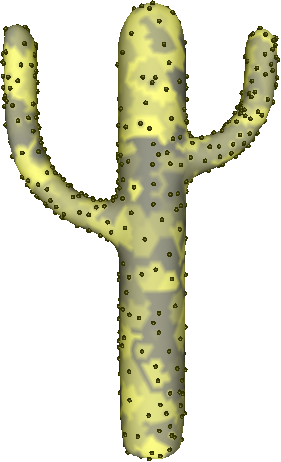
\includegraphics[width=2.0cm]{figs/srarapA.png} & 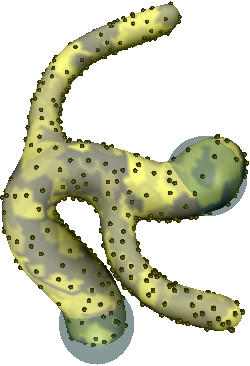
\includegraphics[width=2.0cm]{figs/srarapB.png} & 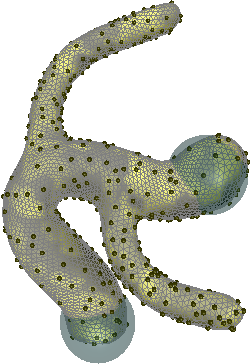
\includegraphics[width=2.0cm]{figs/srarapC.png}\\
% \end{tabular}
% \end{center}
% \caption{SR-ARAP clusters: Left: Hi-res cactus model with Low-res points marked. Clusters formed around vertices are colored with same intensity. 
% Middle and Right deformation of Low-res model transferred to Hi-res model.} 
% \label{fig:SplineAlignedDeformation}
% \end{figure}


% \begin{eqnarray*}
% \sum_{(i,j) \in \mathcal E_i} { c_{ij} q_{ij} } = \sum_{(i,j) \in \mathcal E_i} { \frac{c_{ij}}{2} (R_i p_{ij} \tilde  R_i + R_j p_{ij} \tilde R_j) }
% \end{eqnarray*}
% which can be expressed in matrix form as $\mathrm L Q = C$, where $\mathrm L$ is the symmetric Laplace-Beltrami operator, $Q$ is the column of target positions and $C$ is the right hand side of Equation (\ref{eq:ls_for_p_ga}).

\section{Experiments}

Accuracy, efficiency, with/o noise

\section{Comparisons}

Comparisons with SVD, Horn, Flae, Valkenburg, E3GA. Accuracy, efficiency, with/o noise

\section{C++ code}

%\begin{lstlisting}[language=C++, caption=C++ code for rotor estimation, numbers=left, basicstyle=\tiny, keywordstyle=\bfseries, label=lst:cppcode, morekeywords={Matrix4d,Vector4d,Vector3d,vector,rotor,sqrt}]
\begin{lstlisting}[language=C++, caption=C++ code for rotor estimation, basicstyle=\tiny, keywordstyle=\bfseries, label=lst:cppcode, morekeywords={Matrix4d,Vector4d,Vector3d,Quaterniond,sqrt}]
Quaterniond FastRotorEstimator(
	vector<Vector3d>& P, vector<Vector3d>& Q, vector<double>& weights)
{
	Matrix4d H;
	Vector4d g, R, R_i;
	Vector3d S, D;
	const double epsilon = 1e-6;
	double wj;
	const size_t N = P.size();

	H.setZero();
	for (size_t j = 0; j < N; ++j) {
		wj = weights[j];
		S = Q[j] + P[j];
		D = P[j] - Q[j];
		H(0, 0) += wj*(D[0]*D[0] + D[1]*D[1] + D[2]*D[2]);
		H(0, 1) += wj*(D[0]*S[1] - D[1]*S[0]);
		H(0, 2) += wj*(D[0]*S[2] - D[2]*S[0]);
		H(0, 3) += wj*(D[1]*S[2] - D[2]*S[1]);
		H(1, 1) += wj*(S[1]*S[1] + S[0]*S[0] + D[2]*D[2]);
		H(1, 2) += wj*(S[1]*S[2] - D[2]*D[1]);
		H(1, 3) += wj*(D[2]*D[0] - S[0]*S[2]);
		H(2, 2) += wj*(S[2]*S[2] + S[0]*S[0] + D[1]*D[1]);
		H(2, 3) += wj*(S[0]*S[1] - D[1]*D[0]);
		H(3, 3) += wj*(S[2]*S[2] + S[1]*S[1] + D[0]*D[0]);
	}
	H(1, 0) = H(0, 1);
	H(2, 0) = H(0, 2); H(2, 1) = H(1, 2);
	H(3, 0) = H(0, 3); H(3, 1) = H(1, 3); H(3, 2) = H(2, 3);
	g = -H.col(0);
	H(0, 0) += epsilon; H(1, 1) += epsilon; 
	H(2, 2) += epsilon; H(3, 3) += epsilon;
	H = H.inverse();
	R(0) = 1; R(1) = 0; R(2) = 0; R(3) = 0;
	do {
		R_i = R;
		R(0) -= 1.0;
		R.noalias() = H * (g + epsilon * R);
		R(0) += 1.0;
		R /= sqrt(R.dot(R));
	} while ((R_i - R).dot(R_i - R) > 1e-6);
	return Quaterniond(R(0), -R(3), R(2), -R(1));
}
\end{lstlisting}

\begin{lstlisting}[language=C++, caption=C++ code for rotor estimation using Newton method, basicstyle=\tiny, keywordstyle=\bfseries, label=lst:cppcode_e3ga, morekeywords={Matrix4d,Vector4d,Vector3d,Quaterniond,sqrt}]
Quaterniond RotorEstimator(
	vector<Vector3d>& P, vector<Vector3d>& Q, vector<double>& weights)
{
	const size_t MAX_VECTORS = 32;
	const size_t N = P.size() < MAX_VECTORS? P.size() : MAX_VECTORS;
	Matrix4d Jt[MAX_VECTORS], H;
	Vector4d Fi, g, Ri, R(1, 0, 0, 0);
	Vector3d D, S;
	double wi;

	H.setZero();
	for (size_t i = 0; i < N; ++i) {
		wi = weights[i];
		S = Q[i] + P[i];
		D = P[i] - Q[i];
		Matrix4d& Jti = Jt[i];
		Jti(0, 0) = wi*D[0];  Jti(0, 1) = wi*D[1];  
		Jti(0, 2) = wi*D[2];  Jti(0, 3) = 0;
		Jti(1, 0) = wi*S[1];  Jti(1, 1) = -wi*S[0]; 
		Jti(1, 2) = 0;        Jti(1, 3) = wi*D[2];
		Jti(2, 0) = wi*S[2];  Jti(2, 1) = 0;        
		Jti(2, 2) = -wi*S[0]; Jti(2, 3) = -wi*D[1];
		Jti(3, 0) = 0;        Jti(3, 1) = wi*S[2];  
		Jti(3, 2) = -wi*S[1]; Jti(3, 3) = wi*D[0];
		H(0, 0) += wi*(D[0]*D[0] + D[1]*D[1] + D[2]*D[2]);
		H(0, 1) += wi*(D[0]*S[1] - D[1]*S[0]); 
		H(0, 2) += wi*(D[0]*S[2] - D[2]*S[0]); 
		H(0, 3) += wi*(D[1]*S[2] - D[2]*S[1]);
		H(1, 1) += wi*(S[1]*S[1] + S[0]*S[0] + D[2]*D[2]); 
		H(1, 2) += wi*(S[1]*S[2] - D[2]*D[1]); 
		H(1, 3) += wi*(D[2]*D[0] - S[0]*S[2]);
		H(2, 2) += wi*(S[2]*S[2] + S[0]*S[0] + D[1]*D[1]); 
		H(2, 3) += wi*(S[0]*S[1] - D[1]*D[0]);
		H(3, 3) += wi*(S[2]*S[2] + S[1]*S[1] + D[0]*D[0]);
	}
	H(1, 0) = H(0, 1);
	H(2, 0) = H(0, 2); H(2, 1) = H(1, 2);
	H(3, 0) = H(0, 3); H(3, 1) = H(1, 3); H(3, 2) = H(2, 3);
	H(0, 0) += 1e-6; H(1, 1) += 1e-6; 
	H(2, 2) += 1e-6; H(3, 3) += 1e-6;
	H = H.inverse();
	do {
		Ri = R;
		g.setZero();
		for (size_t i = 0; i < N; ++i) {
			S = Q[i] + P[i];
			D = P[i] - Q[i];
			Fi(0) = -( S[2]*R[2] + S[1]*R[1] + D[0]*R[0]);
			Fi(1) = -( S[2]*R[3] - S[0]*R[1] + D[1]*R[0]);
			Fi(2) = -(-S[1]*R[3] - S[0]*R[2] + D[2]*R[0]);
			Fi(3) = -( D[0]*R[3] - D[1]*R[2] + D[2]*R[1]);
			g += Jt[i] * Fi;
		}
		R += H * g;
		R /= sqrt(R.dot(R));
	} while ((Ri - R).dot(Ri - R) > 1e-6);
	return Quaterniond(R[0], -R[3], R[2], -R[1]);
}
\end{lstlisting}


\bibliographystyle{abbrv}
\bibliography{rotorestimation}

% ------------------------------------------------------------------------
\end{document}
% ------------------------------------------------------------------------
